\documentclass[base]{subfiles}

\begin{document}
\section{Hyperparameters}\label{app:c}

In Figure \ref{fig:mc_rr1}, for a replay ratio of $1$, we display the results of our performance comparison of RDE with SAC using $N=2$ agents with the naive reset and baseline SAC algorithms.

\begin{figure}[h!]
	\centering
	\caption{Performance Comparison in the \texttt{Mountain Car Continuous} Setting when RR=1}
	\label{fig:mc_rr1}
	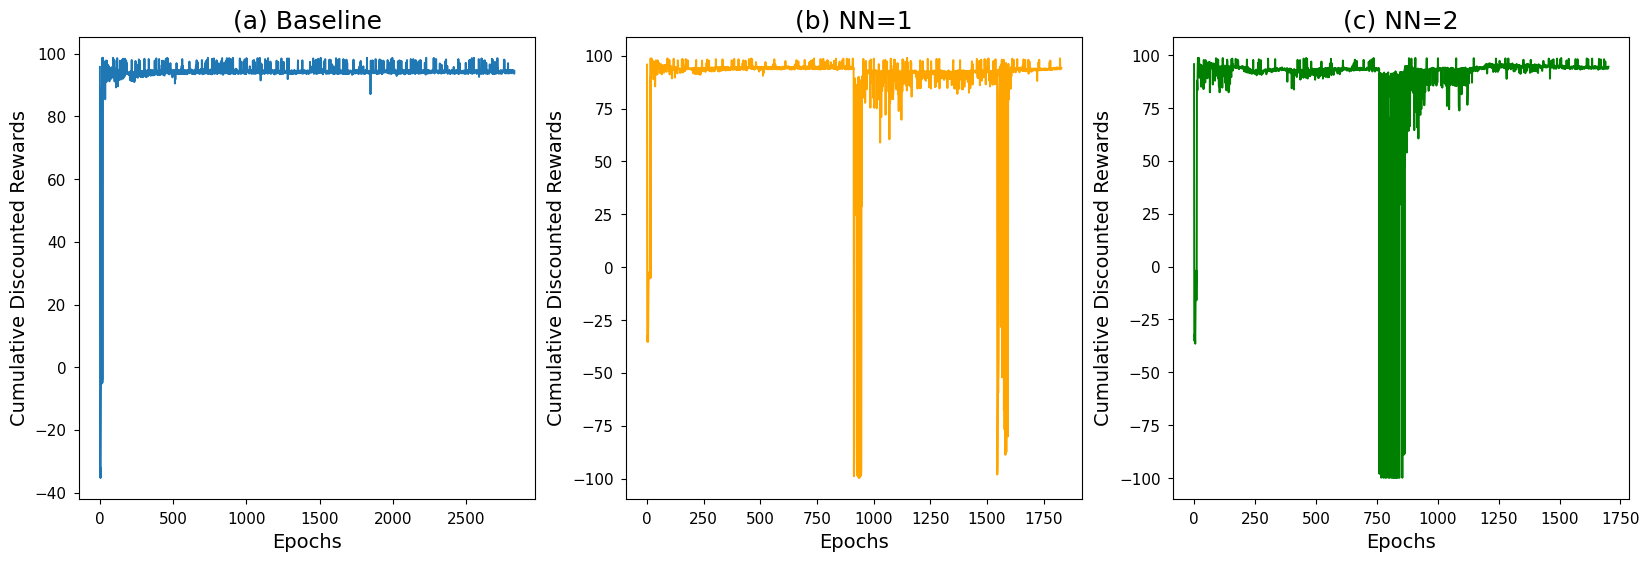
\includegraphics[width = 1 \linewidth]{mc_RR1.png}
	\begin{flushleft} This figure displays our results in the \texttt{Mountain Car Continuous} setting for SAC. We make comparisons across the baseline case, with naive resets with one agent, and with ensemble agents using RDE with two agents. \end{flushleft}
\end{figure}

Next, in Figure \ref{fig:mc_rr4}, we show the results of our performance comparison when the replay ratio is $4$.

\begin{figure}[h!]
	\centering
	\caption{Performance Comparison in the \texttt{Mountain Car Continuous} Setting when RR=4}
	\label{fig:mc_rr4}
	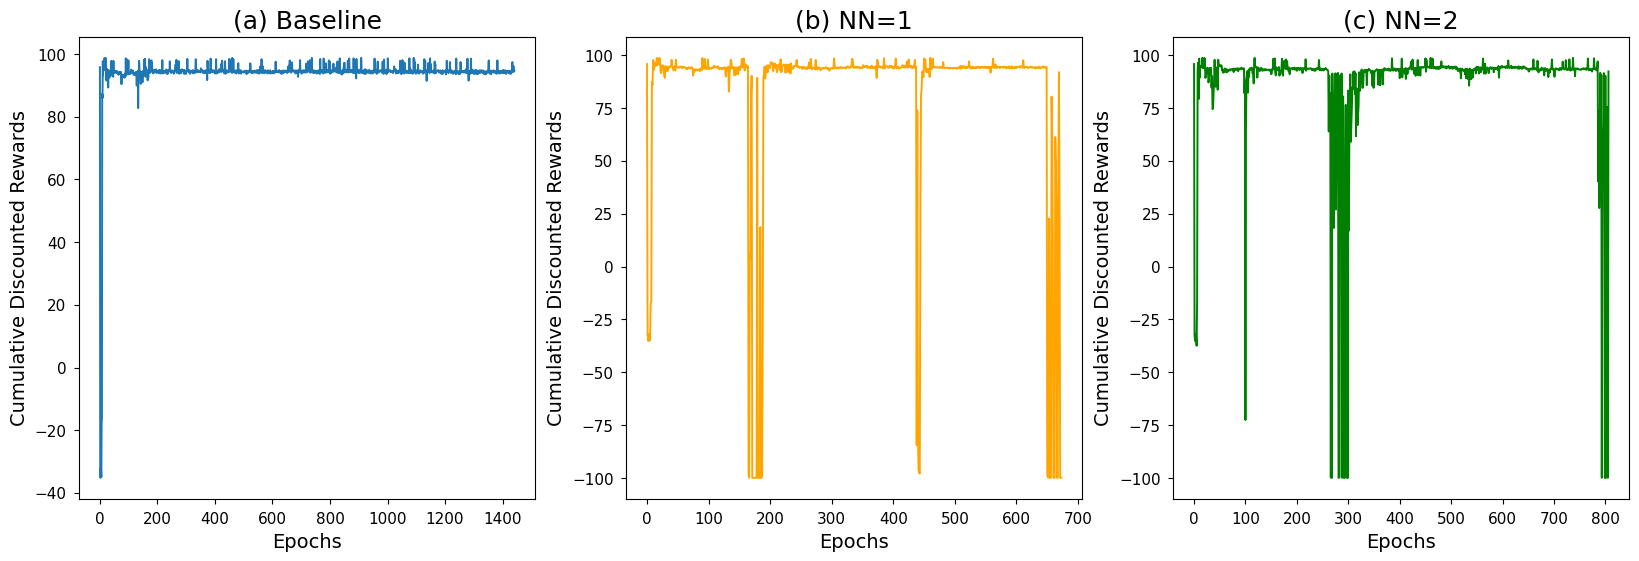
\includegraphics[width = 1 \linewidth]{mc_RR4.png}
	\begin{flushleft} We compare the performance of SAC with a replay ratio of four in the \texttt{Mountain Car Continuous} across the baseline case, with naive resets with one agent, and with ensemble agents using RDE with two agents. \end{flushleft}
\end{figure}

\clearpage

Next, in Figures \ref{fig:cp_rr1} and \ref{fig:cp_rr4}, we display our results for replay ratios of $1$ and $4$ in the \texttt{Cart Pole} environment.

\begin{figure}[h!]
	\centering
	\caption{Performance Comparison in the \texttt{Cart Pole} Setting when RR=1}
	\label{fig:cp_rr1}
	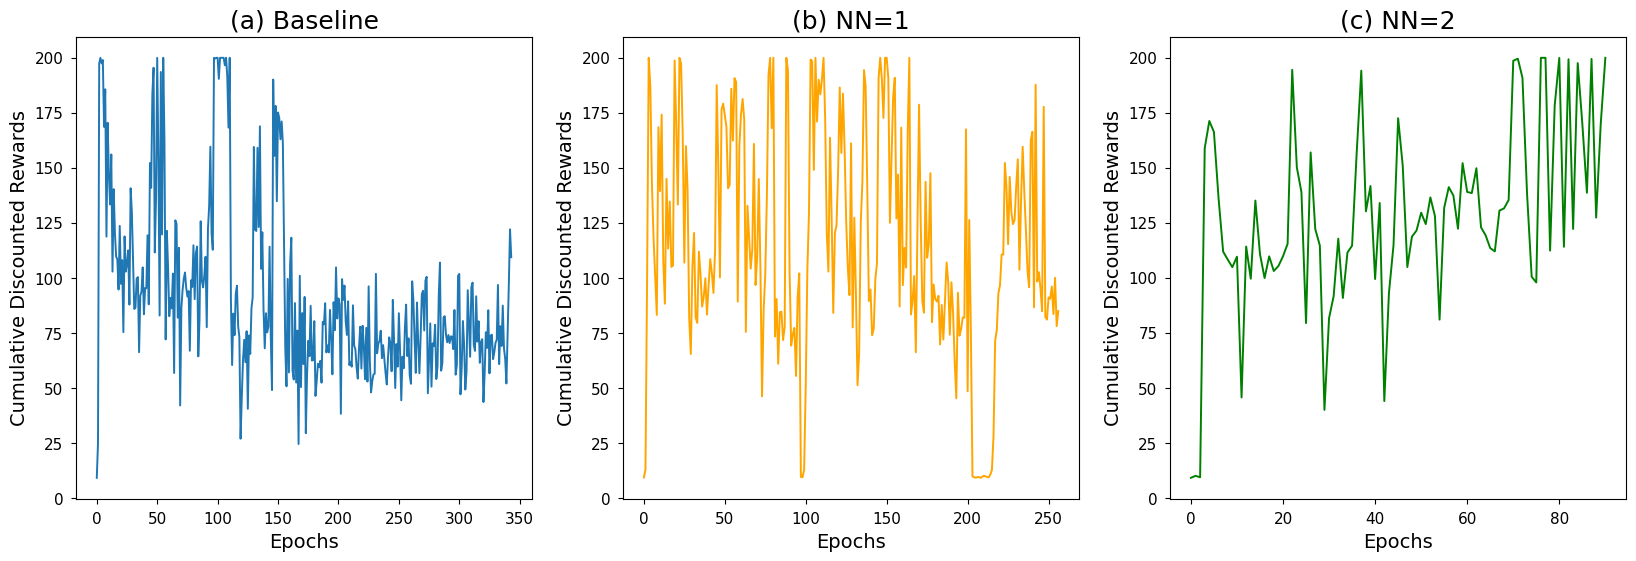
\includegraphics[width = 1 \linewidth]{cp_RR1.png}
	\begin{flushleft} For a replay ratio of one, we compare performance in the \texttt{Cart Pole} setting for DQN. We consider the baseline case, with naive resets with one agent, and with ensemble agents using RDE with two agents. \end{flushleft}
\end{figure}

\begin{figure}[h!]
	\centering
	\caption{Performance Comparison in the \texttt{Cart Pole} Setting when RR=4}
	\label{fig:cp_rr4}
	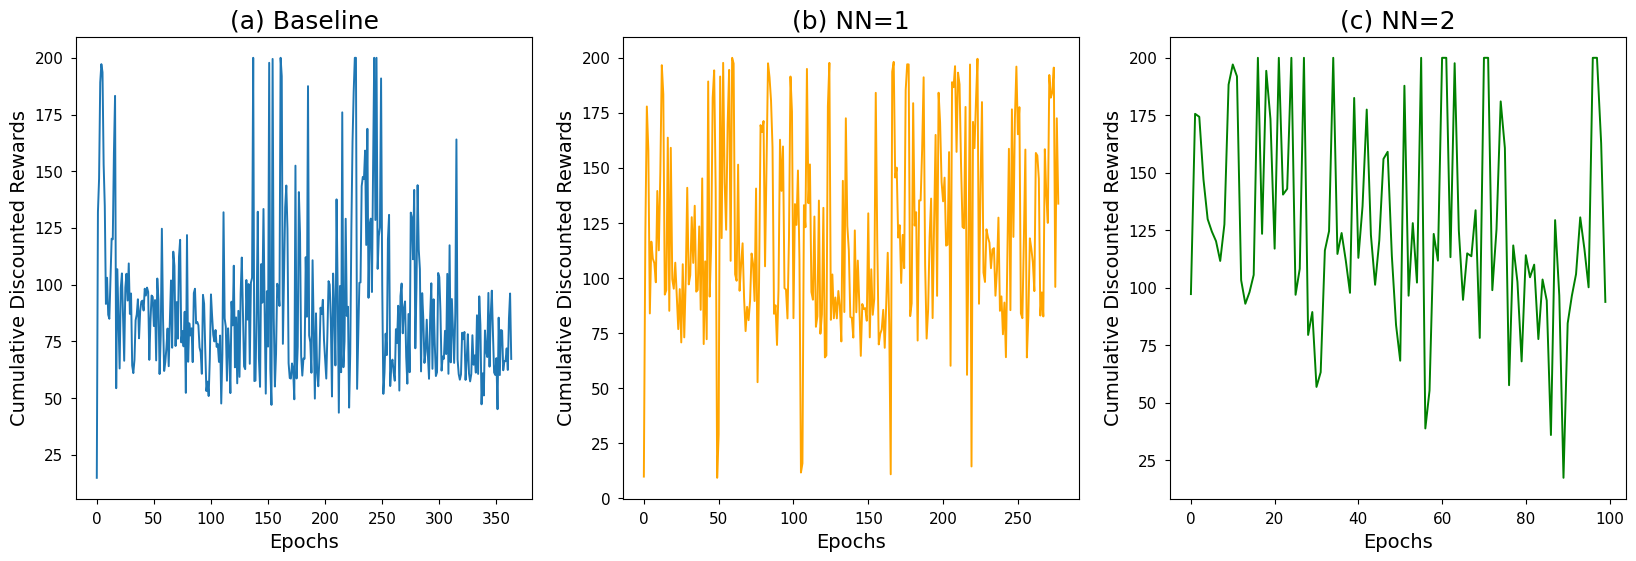
\includegraphics[width = 1 \linewidth]{cp_RR4.png}
	\begin{flushleft} We display our results in the \texttt{Cart Pole} setting for DQN when the replay ratio is four. We examine the baseline case, with naive resets with one agent, and with ensemble agents using RDE with two agents. \end{flushleft}
\end{figure}

\end{document}